\documentclass[a4paper, 12pt]{extarticle}


\usepackage{arxiv}

\usepackage[T2A]{fontenc}
\usepackage[utf8]{inputenc}
\usepackage[english, russian]{babel}
% \usepackage{cmap}
\usepackage{url}
\usepackage{booktabs}
\usepackage{nicefrac}
\usepackage{microtype}
\usepackage{lipsum}
\usepackage{graphicx}
\usepackage{epstopdf}
\usepackage{subfig}
\usepackage[square,sort,comma,numbers]{natbib}
\usepackage{doi}
\usepackage{multicol}
\usepackage{multirow}
\usepackage{tabularx}
\usepackage{float}
\usepackage{amssymb}

\usepackage{tikz}
\usetikzlibrary{matrix}

% Algorithms
\usepackage{algpseudocode}
\usepackage{algorithm}

%% Шрифты
\usepackage{euscript} % Шрифт Евклид
\usepackage{mathrsfs} % Красивый матшрифт
\usepackage{extsizes} % Возможность сделать 14-й шрифт
\usepackage{bm}

\usepackage{makecell} % diaghead in a table
\usepackage{amsmath,amsfonts,amssymb,amsthm,mathtools,dsfont}
\usepackage{icomma}
\usepackage[labelfont=bf]{caption}
\usepackage{subfig} % for subfigures
\usepackage{wrapfig}

\newcommand{\bz}{\mathbf{z}}
\newcommand{\bx}{\mathbf{x}}
\newcommand{\by}{\mathbf{y}}
\newcommand{\bv}{\mathbf{v}}
\newcommand{\bw}{\mathbf{w}}
\newcommand{\ba}{\mathbf{a}}
\newcommand{\bb}{\mathbf{b}}
\newcommand{\bp}{\mathbf{p}}
\newcommand{\bq}{\mathbf{q}}
\newcommand{\bt}{\mathbf{t}}
\newcommand{\bu}{\mathbf{u}}
\newcommand{\bs}{\mathbf{s}}
\newcommand{\bT}{\mathbf{T}}
\newcommand{\bX}{\mathbf{X}}
\newcommand{\bZ}{\mathbf{Z}}
\newcommand{\bS}{\mathbf{S}}
\newcommand{\bH}{\mathbf{H}}
\newcommand{\bW}{\mathbf{W}}
\newcommand{\bY}{\mathbf{Y}}
\newcommand{\bU}{\mathbf{U}}
\newcommand{\bQ}{\mathbf{Q}}
\newcommand{\bP}{\mathbf{P}}
\newcommand{\bA}{\mathbf{A}}
\newcommand{\bB}{\mathbf{B}}
\newcommand{\bC}{\mathbf{C}}
\newcommand{\bE}{\mathbf{E}}
\newcommand{\bF}{\mathbf{F}}
\newcommand{\bomega}{\boldsymbol{\omega}}
\newcommand{\btheta}{\boldsymbol{\theta}}
\newcommand{\bgamma}{\boldsymbol{\gamma}}
\newcommand{\bdelta}{\boldsymbol{\delta}}
\newcommand{\bPsi}{\boldsymbol{\Psi}}
\newcommand{\bpsi}{\boldsymbol{\psi}}
\newcommand{\bxi}{\boldsymbol{\xi}}
\newcommand{\bchi}{\boldsymbol{\chi}}
\newcommand{\bzeta}{\boldsymbol{\zeta}}
\newcommand{\blambda}{\boldsymbol{\lambda}}
\newcommand{\beps}{\boldsymbol{\varepsilon}}
\newcommand{\bZeta}{\boldsymbol{Z}}
% mathcal
\newcommand{\cX}{\mathcal{X}}
\newcommand{\cY}{\mathcal{Y}}
\newcommand{\cW}{\mathcal{W}}

\newcommand{\dH}{\mathds{H}}
\newcommand{\dR}{\mathds{R}}
% transpose
\newcommand{\T}{^{\mathsf{T}}}

% \renewcommand{\shorttitle}{\textit{arXiv} Шаблон}
\renewcommand{\epsilon}{\ensuremath{\varepsilon}}
\renewcommand{\phi}{\ensuremath{\varphi}}
\renewcommand{\kappa}{\ensuremath{\varkappa}}
\renewcommand{\le}{\ensuremath{\leqslant}}
\renewcommand{\leq}{\ensuremath{\leqslant}}
\renewcommand{\ge}{\ensuremath{\geqslant}}
\renewcommand{\geq}{\ensuremath{\geqslant}}
\renewcommand{\emptyset}{\varnothing}

\DeclareMathOperator*{\argmax}{arg\,max}  % in your preamble
\DeclareMathOperator*{\argmin}{arg\,min}  % in your preamble 

\usepackage{hyperref}
% \usepackage[usenames,dvipsnames,svgnames,table,rgb]{xcolor}

\hypersetup{
	unicode=true,
	pdftitle={A template for the arxiv style},
	pdfsubject={q-bio.NC, q-bio.QM},
	pdfauthor={David S.~Hippocampus, Elias D.~Striatum},
	pdfkeywords={First keyword, Second keyword, More},
	colorlinks=true,
	linkcolor=black,        % внутренние ссылки
	citecolor=blue,         % на библиографию
	filecolor=magenta,      % на файлы
	urlcolor=blue           % на URL
}

\graphicspath{{./figures}}

\usepackage{enumitem} % Для модификаций перечневых окружений

\theoremstyle{definition} % "Определение"
\newtheorem{definition}{Опр.}[section]

\usepackage{etoolbox}

\makeatletter
\expandafter\patchcmd\csname\string\algorithmic\endcsname{\itemsep\z@}{\itemsep=1.5mm}{}{}
\makeatother

\newcommand{\myfigref}[2]{~\ref{#1}.\subref{#2}}% <---- a new macro for referring to a subfigure
\renewcommand{\abstractname}{Аннотация}

\title{Пространственно-временные характеристики в задаче декодирования временных рядов.}

\author{
	Дорин Даниил \\
	\texttt{dorin.dd@phystech.edu} \\
	\And
	Грабовой Андрей \\
	\texttt{grabovoy.av@phystech.edu}
}
\date{\today}

\begin{document}
\maketitle

\begin{abstract}

	Исследуются пространственно-временные характеристики в задаче декодирования временных рядов с дискретным представлением времени.
	В качестве задачи декодирования рассматривается задача классификации сигнала. 
	В работе проводится обзор методов классификации регестрируемого сигнала. 
	Предлагается метод классификации временных рядов, основанный на применении Римановой геометрии. 
	Для анализа предложенного метода проводится вычислительный эксперимент на выборке, 
	полученной при исследовании электрической активности мозга большого числа испытуемых с применением неинвазивной электроэнцефалографии. 
	Для увеличения объема выборки производится аугментация данных. 
	Проводится сравнение предложенного метода с известными методами классификации электроэнцефалограмм, полученных при регистрации колебаний электрического 
	потенциала головного мозга через покровы головы.

\end{abstract}

\keywords{ЭЭГ \and временные ряды \and Риманова геометрия \and пространственно-временные характеристики \and декодирование \and классификация}

\section{Введение}

\indent Основной целью анализа сигнала в данном исследовании является 
классификация электроэнцефалограммы (ЭЭГ) \citep{teplan2002fundamentals, beniczky2020electroencephalography}~--- раздел электрофизиологии, 
изучающий закономерности суммарной электрической активности мозга, 
отводимой с поверхности кожи волосистой части головы, 
а также метод записи таких потенциалов. Также ЭЭГ~--- неинвазивный метод, то есть 
не требует проникновения внутрь организма или повреждения кожи или других тканей. 
Вместо этого, данные собираются с помощью внешних средств. 
В последнее время активно ведутся научные исследования, 
посвященные методам регисттрации активности мозга и декодированию 
информации \citep{siuly2016eeg, craik2019deep}. Основным направлением применения 
этих методов являются технологии нейрокомпьютерных интерфейсов.

Исследования ЭЭГ широко используются в медицинской практике для диагностики 
различных состояний мозга. Проведение классификации сигналов ЭЭГ играет важную роль в определении 
уровня болезни, выявлении эпилептических припадков, оценке состояния пациента в коме, а 
также для мониторинга глубокого сна \citep{smith2005eeg, gajic2014classification}.

Одним из успешных традиционных методов классификации наличия потенциала P300 на электроэнцефалограмме (ЭЭГ) является
алгоритм \textbf{ERPCov TS}. Под потенциалом P300 понимается связанный с 
событием (event-related potential — ERP) измеренный отклик мозга, 
который является прямым результатом определенного ощущения, 
когнитивного или моторного события.
Алгоритм основан на применении Римановой геометрии \citep{barachant2010riemannian}. 
Первым этапом данного алгоритма является формирование пространства центрированных признаков.

\begin{equation*}
	\bm{X}_i= \left[\bm{x}^i_1,\dots \bm{x}^i_{T}\right] = 
	\begin{bmatrix}
	x^i_{1,1} & x^i_{1,2} &  \dots  &  x^i_{1,T}\\
	\dots & \dots &  \dots  &  \dots\\
	x^i_{K,1} & x^i_{K,2} &  \dots  &  x^i_{K,T}
	\end{bmatrix}
	= \begin{bmatrix}
		ts_1\\
		\dots\\
		ts_K
		\end{bmatrix},
	\end{equation*}
где $ts_j$ ~--- временной ряд с нулевым средним, полученный при измерении сигнала $j$-ым датчиком и последующего центрирования.
Тогда ковариационная матрица для одного измерения ЭЭГ имеет вид:
$$\bm{R}_i = \dfrac{1}{T-1}\bm{X}_i\bm{X}_i^{\T}, ~\bm{R} \in \mathbb{R}^{K\times K},~i = \overline{1, N}$$

Для классификации потенциала P300 в алгоритме используется расширенная матрица ковариации:
$$\bm{R}_i = \dfrac{1}{T-1} \bm{P}_i\bm{P}_i^{\T},~\bm{P}_i = \begin{bmatrix}
	\overline{\bm{X}^0}\\
	\overline{\bm{X}^1}\\
	\bm{X}_i
	\end{bmatrix},$$
где $\overline{\bm{X}^c}$ и $\overline{\bm{X}^1}$~--- средние по классам $\{0,1\}$ значения:
$$\overline{\bm{X}^0} = \dfrac{\sum_{i = 1}^N\left[y_i = c\right] \bm{X}_i}{\sum_{i = 1}^N\left[y_i = c\right]},~c\in\{0,1\}$$
Известно, что пространство, состоящее из матриц ковариации, представляет собой 
Риманово многообразие\citep{barachant2010riemannian}. 
В каждой точке данного риманова многообразия имеется касательная плоскость с 
определенным скалярным произведением на ней. Общая касательная плоскость, 
предназначенная для отображения всех матриц ковариации в выборке, 
формируется в точке среднего геометрического по римановой метрике 
известных ковариационных матриц. Среднее геометрическое симметричных положительно определенных матриц имеет вид:
$$\bm{R} = \mathfrak{G}\left(\bm{R}_1,\dots,\bm{R}_N\right) = \underset{\bm{R}}{\text{argmin}}\sum_{i = 1}^N
\delta^2_R(\bm{R},~\bm{R}_i),$$
где риманова метрика определяется следующим образом (геодезическое расстояние):
$$\delta_R(\bm{R},~\bm{R}_i) = \|\log (\bm{R}^{-1}\bm{R}_i)\|_F = \sqrt{\sum_{i = 1}^{3N} \log^2\lambda_i},$$
где $\lambda_i$~--- собственные значения матрицы $\bm{R}^{-1}\bm{R}_i$. В работе \citep{barachant2010riemannian}
получено, что для каждой ковариационной матрицы $\bm{R}_i$ существует проекция $\bm{\pi}_i$ на касательное пространство.
Таким образом, определено отображение:
$$\text{Exp}_{R}(\bm{\pi}_i) = \bm{R}_i = \bm{R}^{\frac{1}{2}} \exp\left(\bm{R}^{-\frac{1}{2}}\bm{\pi}_i\bm{R}^{-\frac{1}{2}}\right) \bm{R}^{\frac{1}{2}}$$
$$\log_{R}(\bm{R}_i) = \bm{\pi}_i = \bm{R}^{\frac{1}{2}} \log\left(\bm{R}^{-\frac{1}{2}}\bm{R}_i\bm{R}^{-\frac{1}{2}}\right) \bm{R}^{\frac{1}{2}}$$

На практике построение ковариационных матриц и получение их образов в касательном пространстве выполняется 
при помощи библиотеки \textbf{PyRiemann} \citep{congedo2013new}.

После векторизации полученные данные используются как новое признаковое пространство и 
могут быть классифицированы при помощи классических методов машинного обучения. 

%%%%%%%%%%%%%%%%%%%%%%%%%%%%%%%%%%%%%%%%%%%%%%%%%%%%%%%%%%%%%%%%%%%%%%%%%%%%%%%%%%%%%%%%%
\section{Постановка задачи}
Исследуется задача декодирования временного ряда. Пусть имеется некоторый процесс (активность головного мозга):
$$\mathcal{V}(\tau),~\tau \in \mathbb{R}$$
Тогда данные выборки ~--- это регистрируемый сигнал, то есть реализация процесса $\mathcal{V}(\tau)$:
$$\bm{X} = \left[\bm{x}_1,\dots \bm{x}_{T}\right],~\bm{x}_t \in \mathbb{R}^K$$
Здесь $K$ ~--- число каналов. $T$ ~--- число измерений сигнала с частотой $\mu$ за время $\tau$:
$$T = \tau \mu$$
$$\bm{x}_{\tau \mu} \approx \mathcal{V}(\tau)$$
\subsection{Задача классификации отрезков регистрируемого сигнала}
В данной задаче имеется выборка регистрируемых отрезков сигнала, 
требуется классифицировать каждый наблюдаемый временной отрезок. 
Введем следующие обозначения:
Пусть имеется $N$ зарегистрированных реализаций некоторого процесса:
$$\bm{X} = \{\bm{X}_1,\dots, \bm{X}_N\},$$
$$\bm{X}_i = \left[\bm{x}^i_1,\dots, \bm{x}^i_{T}\right], ~\bm{x}^i_t \in \mathbb{R}^K,$$
$$\bm{Y} = \left[y_1, \dots, y_{N}\right]^{\T},~y_i \in \{1,\dots, C\}$$
Здесь $y_i$~--- целевая метка класса $i$-го зарегистрированного сигнала. $C$ ~--- число классов в задаче классификации сигнала. 

Имеется соответственно выборка $\mathcal{D} = \{y_i, \bm{X}_i\},~  i = \overline{1,N}$
Требуется построить отображение $f_\theta$, которое учитывало 
бы пространственно-временные характеристиик между временными рядами от датчиков:
$$f_\theta: \bm{X} \rightarrow \{1,\dots, C\}$$ 
\subsection{Задача классификации активности}
В данной задаче предполагается получение классификации для каждого отсчета 
времени наблюдения.
Пусть имеется некоторый процесс и зарегистрированная реализация данного 
процесса в виде дискретного числа измерений. Каждому измерению соответствует
класс активности. Формально:
$$\bm{X} = \{\bm{x}_1,\dots, \bm{x}_{T}\}, ~\bm{x}_t \in \mathbb{R}^K,$$
$$\bm{Y} = \left[y_1, \dots, y_{T}\right]^{\T},~y_t \in \{1,\dots, C\}$$
Здесь $C$ ~--- число классов в задаче классификации активности. 
Выборка $\mathcal{D} = \{y_t, \bm{x}_t\}_{t=1}^T$

Для набора данных, описанного выше, требуется построить отображение $f_\theta$, которое учитывало 
бы пространственно-временные характеристиик между временными рядами сигнала:
$$f_\theta: \bm{X} \rightarrow \{1,\dots, C\}$$ 




\section{Вычислительный эксперимент}
\subsection{Первая постановка задачи}
Для анализа работоспособности предложенного метода, а также проверки гипотез
проведен вычислительный эксперимент.

Для проведения экспериментов используется набор данных \citep{schalk2004bci2000} 64-канальных ЭЭГ сигналов от испытуемых, 
выполнявших серию моторных/образных задач. Этот набор данных состоит из более 
чем 1500 одно- и двухминутных записей ЭЭГ, полученных от 109 волонтеров во время выполнение различных заданий. 
 
Для проведения базового эксперимента используется подвыборка для задачи бинарной классификации состояния глаз открыты/закрыты.

\subsection*{Применение Римановой геометрии}
Рассмотрим несколько классических методов классификации. 
Метод опорных векторов~---один из наиболее популярных методов обучения, который применяется для решения задач классификации и регрессии.
Чтобы показать преимущество перехода к Риманову касательному пространству, проведем следующий эксперимент. 
Векторизуем все многомерные временные ряды и обучим на полученных векторах SVM. 
Теперь применим алгоритм векторизации ERPCov TS на многомерных временных рядах, основанный на Римановой геометрии, и после этого обучим SVM на векторизованных данных. 
Результаты на валидации и тесте приведены в таблице \ref{table:Riman}. 
Качество классификации после проектирования на касательное пространство гораздо лучше.

\begin{table}[h!]
	\centering
	\caption{Сравнение методов}
	\begin{tabular}{|c|c|c|}
		\hline
		& \multicolumn{2}{|c|}{accuracy}  \\ \hline 
		Метод & валидация  & тест \\ \hline \hline
		SVM    & $0.732$ & $0.697$      \\ \hline
		ERPCov TS SVM    & $0.939$ & $0.954$		\\ \hline
	\end{tabular}
	\label{table:Riman}
\end{table}



\subsection{Вторая постановка задачи}
Для проведения экспериментов была использована выборка бинарной классификации состояния глаз.
Набор данных получен в результате одного непрерывного измерения неинвазивного ЭЭГ с 
помощью нейроголовки Emotiv EEG с использованием 14 датчиков, на рис.\ref{fig:1} задействованные датчики
изображены красным цветом. 
\begin{figure}[h]
	\centering
	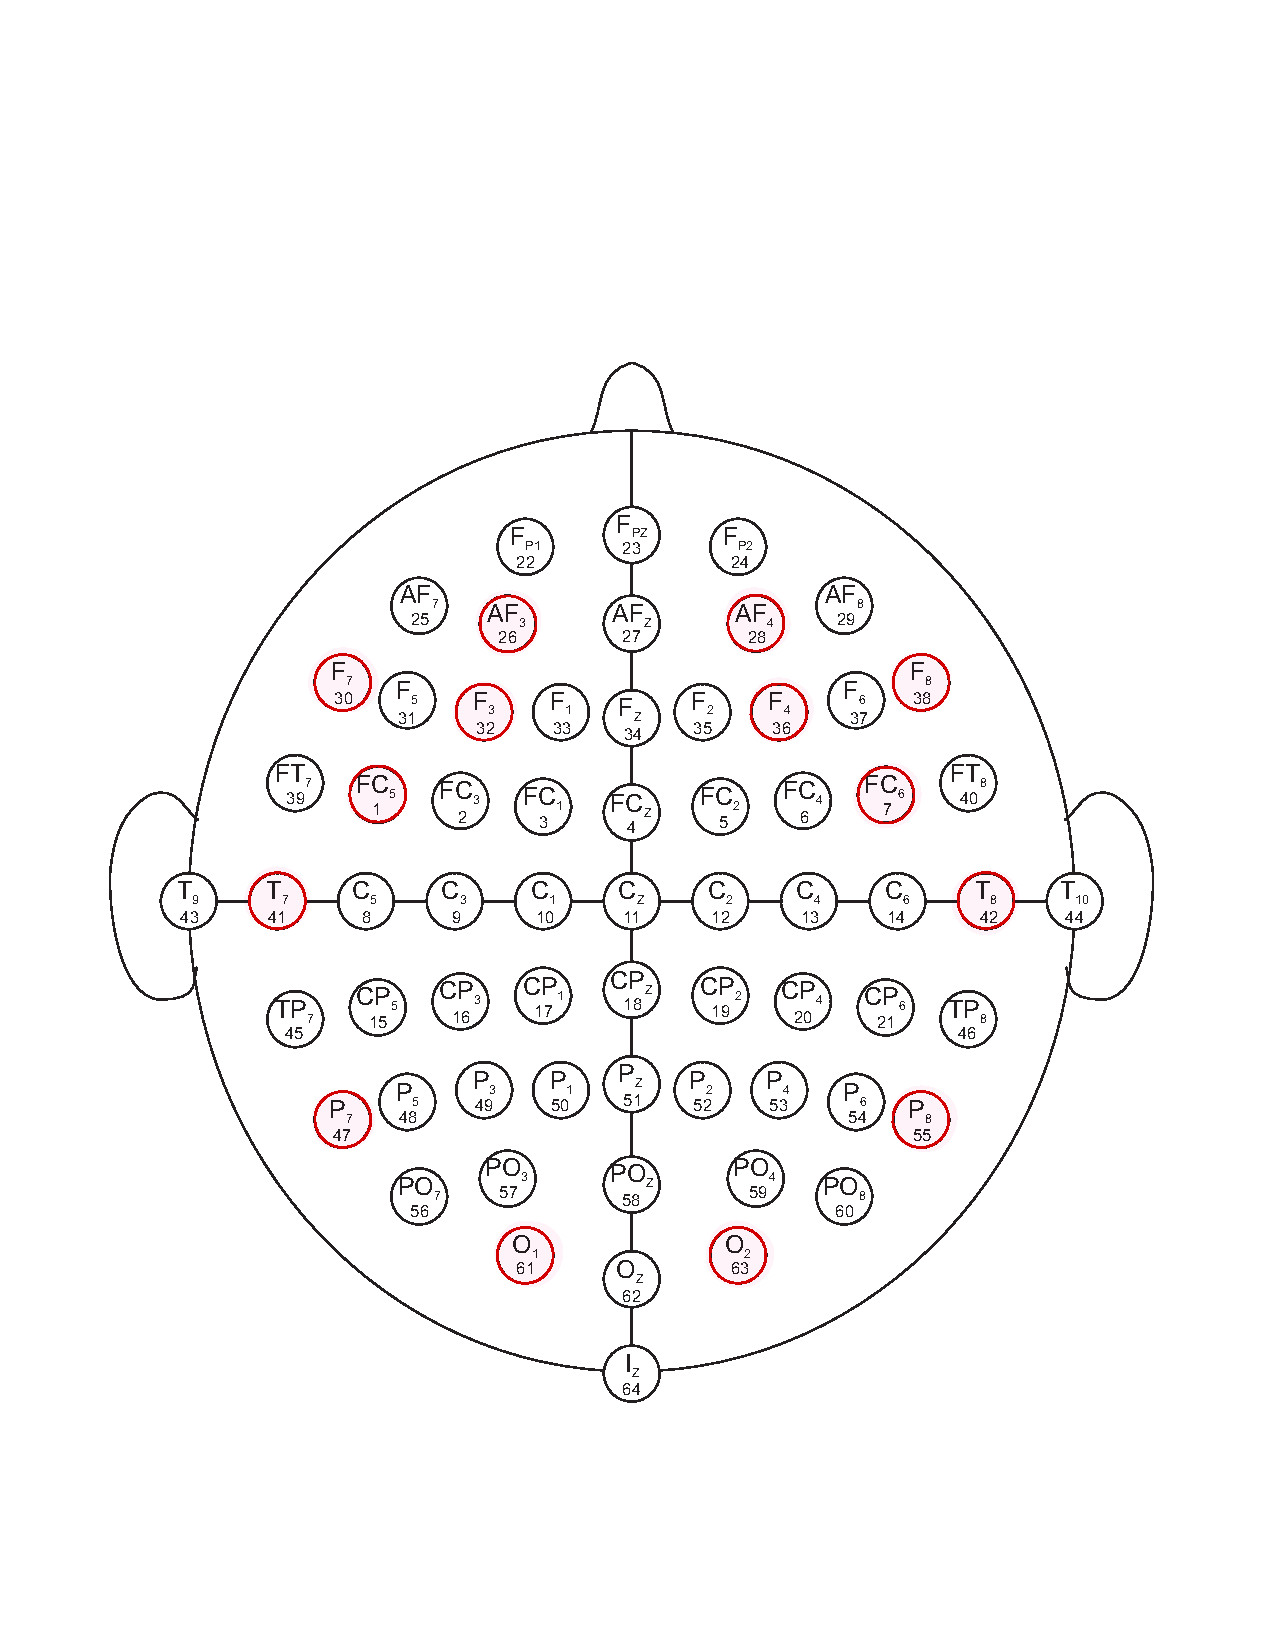
\includegraphics[width=0.75\textwidth]{64_channel_sharbrough.pdf}
	\caption{Задействованные датчики ЭЭГ при измерении сигнала}
	\label{fig:1}
\end{figure}


Продолжительность измерения в выборке составила 117 секунд. 
Состояние глаз было зафиксировано с помощью камеры во время измерения ЭЭГ и позже добавлено 
вручную в файл после анализа видеокадров. Метка <<1>> указывает на состояние с закрытыми глазами, а 
<<0>> ~--- на состояние с открытыми глазами. Все значения приведены в хронологическом порядке с 
первым измеренным значением в верхней части данных.
Основные характеристики выборки представлены в
Таблице~\ref{table:sample}.

\begin{table}
	\centering
	\caption{Описание выборки}
	\begin{tabular}{|c|c|c|}
		\hline
		Название                       & Обозначение & Значение             \\
		\hline \hline
		Продолжительность обследования & $\tau$         & 117 с                \\ \hline
		Частота измерения сигнала      & $\mu$       & 128.03 $\text{с}^{-1}$   \\ \hline
	    Число каналов (датчиков)    & $K$   & 14          \\ \hline
		Число измерений сигнала             & $T$  & 14980           \\ \hline
	\end{tabular}
	\label{table:sample}
\end{table}
При анализе выборки обнаружено 4 выброса, которые были заменены средними по классам 
значениями, график временных рядов после обработки выбросов представлен на рис.\ref{fig:2}.

\begin{figure}[h]
	\centering
	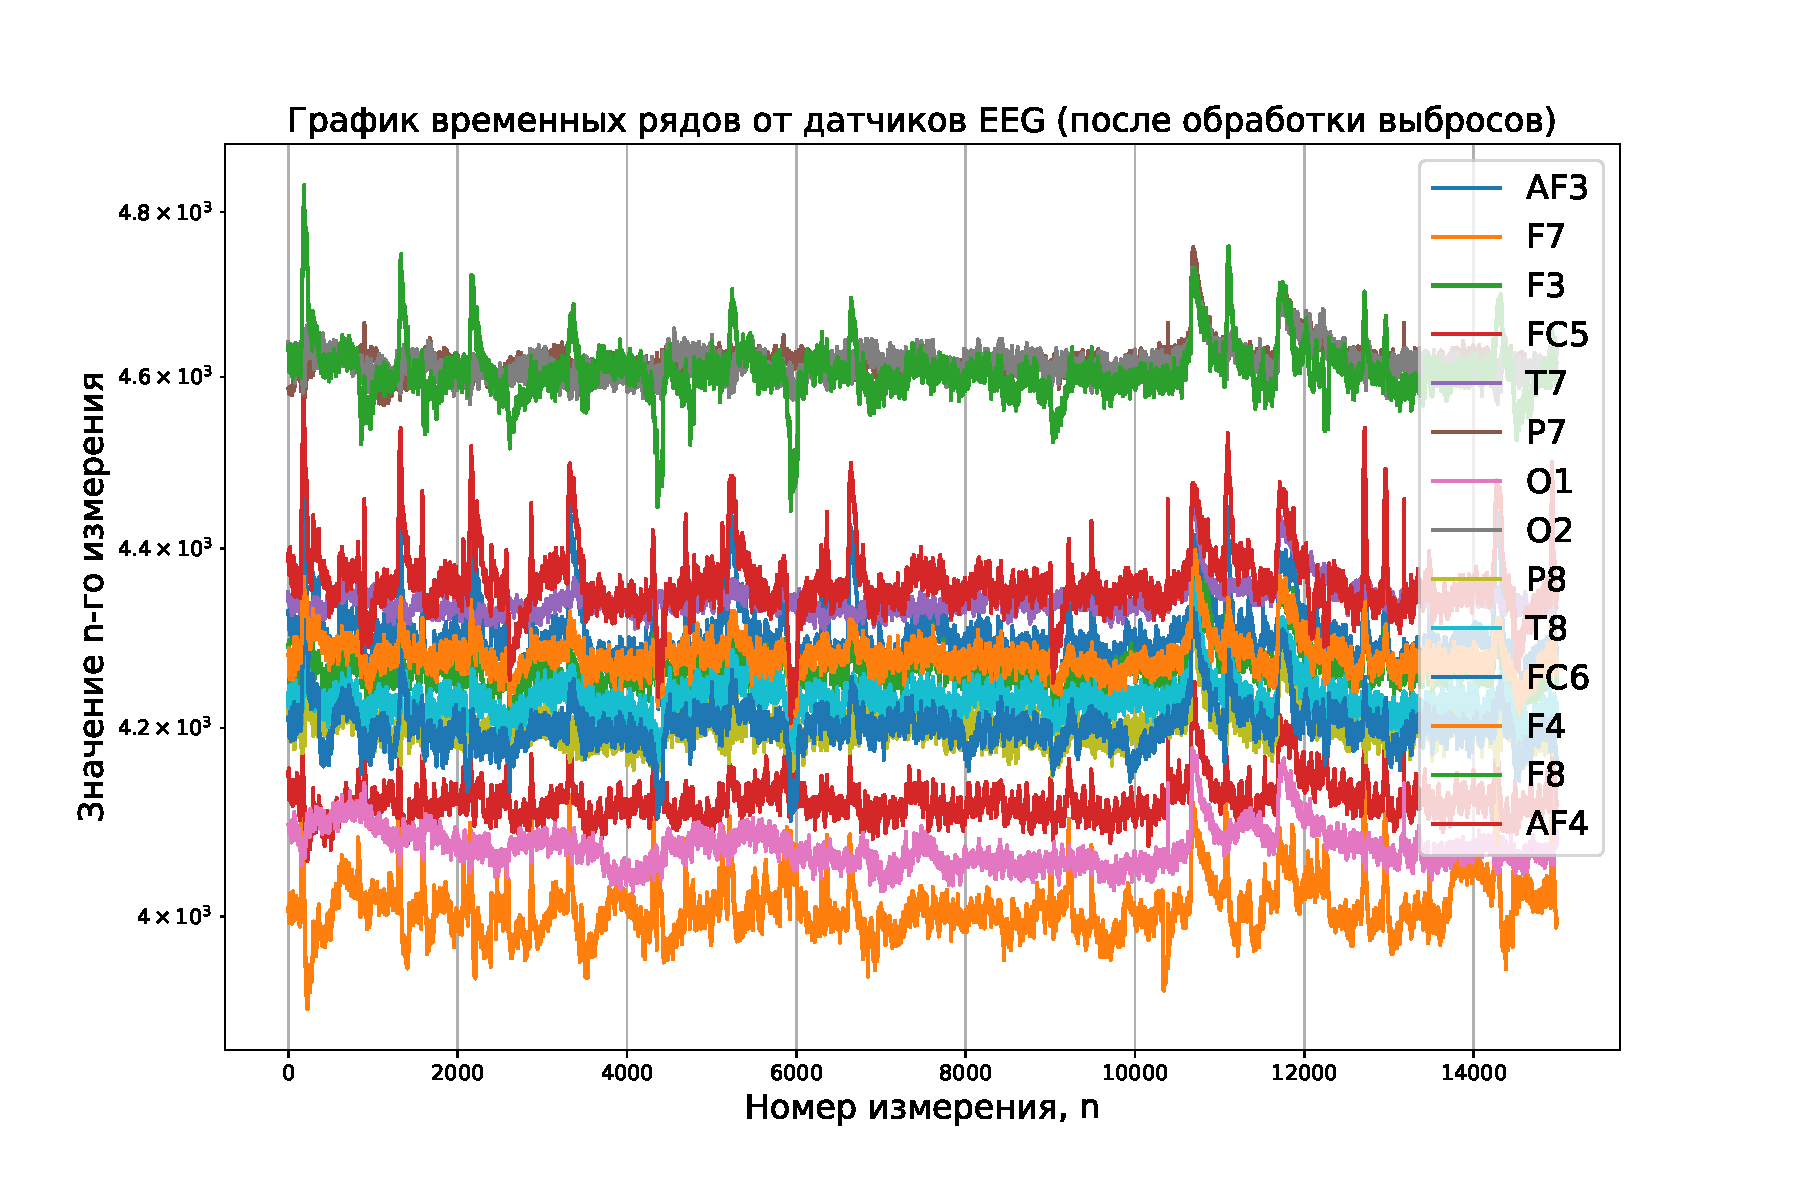
\includegraphics[width=0.8\textwidth]{Dataset.pdf}
	\caption{График временных рядов}
	\label{fig:2}
\end{figure}


\textbf{TODO}: попробовать применить библиотеку \textbf{PyRiemann} к данным.

\section{Заключение}


\newpage

\bibliographystyle{plain}
\bibliography{references.bib}

\end{document}
